\documentclass[]{article}

\usepackage{amssymb}
\usepackage{amstext}
\usepackage{amsthm}
\usepackage{amsmath}
\usepackage{enumerate}
\usepackage{fancyhdr}
\usepackage[margin=1in]{geometry}
\usepackage{graphicx}
\usepackage{extarrows}
\usepackage{setspace}
\usepackage{graphicx}
\usepackage{float}
\usepackage{tocloft}

\pagestyle{plain}
\renewcommand\headrulewidth{0.4pt}
\renewcommand\footrulewidth{0.4pt}

\title{Detailed Design: \\ \textit{IdentiFisher} \\ An Android Application \\}
\author{
\Large McDonald, Christopher\\
\texttt{1312456} \\ \\
\Large Guo, Tian\\
\texttt{1327833} \\ \\
\Large Murray, Shandelle\\
\texttt{1303109} \\ \\
\Large Cheung, Ocean\\
\texttt{1316057} \\
}

\vfill
\date{Last Edited On: \today}

\begin{document}
\maketitle

\newpage

\tableofcontents
\vfill
Revision 0: This is the first draft written from the authors listed on the Title page.
\pagebreak
\section{Introduction}
\label{sec:introduction}

\subsection{Purpose}
\label{sub:purpose}

This document is the third, and final documentation which outlines the details of the ineficaion application IdentiFisher. This document specifically will provide ample detail into the components of the application so that a person with the appropriate expertise could implement it. These details will include the processes of the application, the life cycle of each component and what is expected or required from them. \\
This document is crucial for the project managers and programmers as there will be heavy detail on how the application will execute. However, it is also important for all stakeholders to read this document because of their involvement in the success of the application. These stakeholders should be making sure the application is aligning with the goals and aspirations it had always intended, and provide guidance when necessary.

\subsection{System Description}
\label{sub:system_description}

This system is an Android Application, running on the most up to date Android operating system, Android \textit{Marshmellow}. It will provide the service of indentifying the type of fish a User is describing, when given a required set of criteria. Additional features included tracking the fish that users has caught with the geolocation they are at as well as providing warnings to users if the fish is potentially dangerous or endangered. This requires text input from the user, as well as GPS functionality from the smartphone. Given the information we are holding, we also provide the service to users to look up data for each geolocation they provide. This application will be very easy to use, as fishing can involve varying level of intensity and should be available in all of these times.

\subsection{Overview}
\label{sub:overview}

This documents contains varying levels of detailed design components the implementation must have. The first section to note is Section \ref{sec:state_charts_for_controller_classes} which is the State Charts for Controller Classes. This will be a state machine to describe the action, outputs and states for each Controller class in the application. For reference, the Controller classes can be found in the High Level Architecure Design document. These will be useful to outline how the system acts when given an input during a particular time. Continuing from there in Section \ref{sec:sequence_diagrams} is the Sequence Diagrams. This section is a major aspect of the life cycle of the application in its entirety and also the sub compenents of the application. This diagram will show when processes are started, when they end and what messages or actions are sent between them. This part is crucial to the synchronous aspects of the application. Lastly in Section \ref{sec:detailed_class_diagram} is the Detailed Class Diagram which will take each Class required for the implentation of the program and go into great detail about it. This will include the inputs, resources, expectations and outputs of each class. Moreover, the attributes and methods each class will need should be outlined as well.

\section{State Charts for Controller Classes}
\label{sec:state_charts_for_controller_classes}
In this section, a state chart for each control class will be displayed. The state chart will demonstrate how each classes behave as a result of respective inputs. Note that the Expert classes were combined into one chart as they behave similarly.
\begin{figure}[H]
	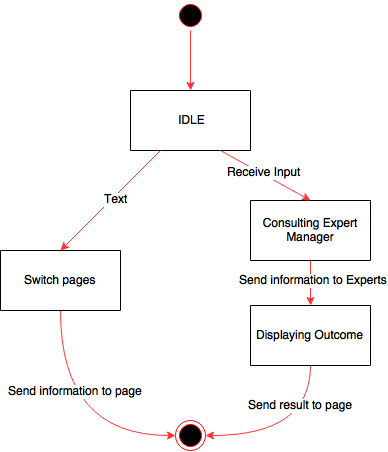
\includegraphics[width=\textwidth]{images/ViewController.png}
	\caption{State Chart: ViewController}
\end{figure}
\begin{figure}[H]
	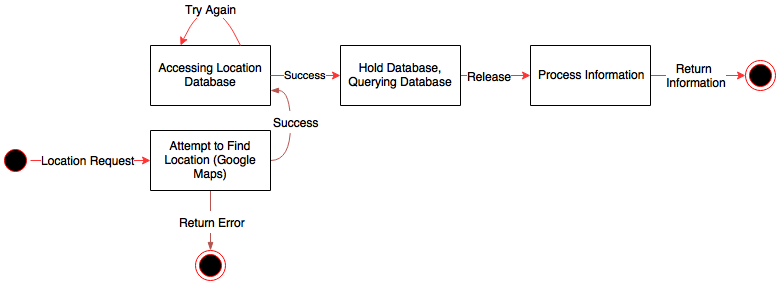
\includegraphics[width=\textwidth]{images/GeoLocation.png}
	\caption{State Chart: GeoLocation}
\end{figure}
\begin{figure}[H]
	\begin{center}
	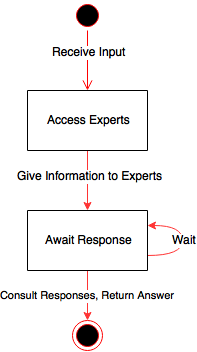
\includegraphics[width=0.5\textwidth]{images/ExpertManager.png}
	\caption{State Chart: Expert Manager}
	\end{center}
\end{figure}
\begin{figure}[H]
	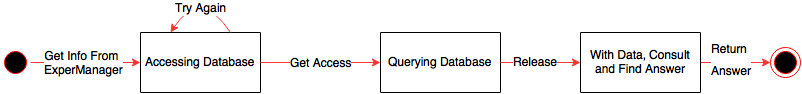
\includegraphics[width=\textwidth]{images/Expert.png}
	\caption{State Chart: Expert}
\end{figure}

\section{Sequence Diagrams}
\label{sec:sequence_diagrams}
% Begin Section
The following sequence diagrams depict use cases of the IdentiFisher application. The first sequence diagram shows the process of a user requesting and the application providing an identification of a fish based on user input. The second sequence diagram shows the user obtaining fish population statistics of a specific lake or body of water. The third sequence diagram shows the user adding a self-identified fish to the database which is tentative until the database administrator confirms the submission. The fourth sequence diagram shows the database administrator updating expert details, which may include adding, deleting, or modifying an expert.
\begin{figure}[H]
	\includegraphics[width=\textwidth]{images/sequence1.png}
	\caption{Sequence Diagram: Fish Identification}
\end{figure}
\begin{figure}[H]
	\includegraphics[width=\textwidth]{images/sequence2.png}
	\caption{Sequence Diagram: Look up Body of Water Statistics}
\end{figure}
\begin{figure}[H]
	\includegraphics[width=\textwidth]{images/sequence3.png}
	\caption{Sequence Diagram: Add Self-Identified Fish to Database}
\end{figure}
\begin{figure}[H]
	\begin{center}
	\includegraphics[width=0.5\textwidth]{images/sequence4.png}
	\caption{Sequence Diagram: Update Experts}
	\end{center}
\end{figure}
% End Section

\section{Detailed Class Diagram}
\label{sec:detailed_class_diagram}
% Begin Section
\begin{figure}[H]
	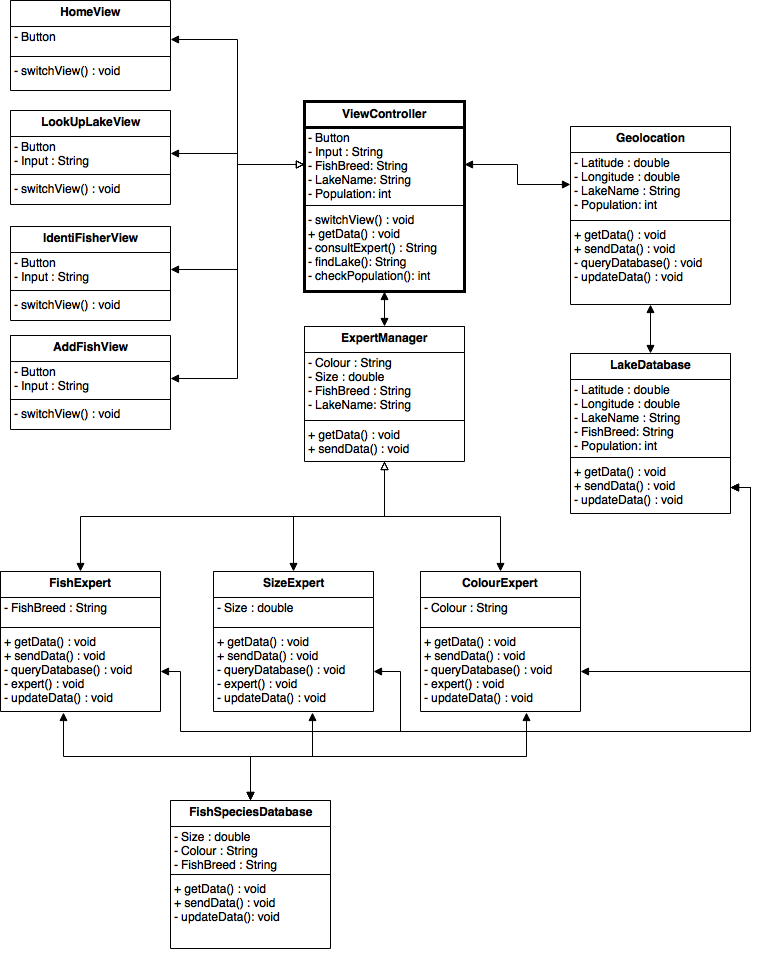
\includegraphics[width=\textwidth]{images/DetailedClassDiagram.png}
	\caption{Detailed Class Diagram}
\end{figure}
% End Section

\vfill
\listoffigures

\appendix
\section{Division of Labour}
\label{sec:division_of_labour}
% Begin Section
\begin{center}
\begin{tabular}{ |c|c|c| }
 \hline
 Name & Labour & Signature \\ \hline
 Shani & Sequence Diagrams & \\
 Chris & Introduction  &  \\
 Ocean &  Detailed Class Diagram &  \\
 Tian & State Charts for Controller Classes & \\
 \hline
\end{tabular}
\end{center}


\end{document}
%------------------------------------------------------------------------------
